\documentclass[12pt]{article} %Styl dokumentu
\usepackage{times} %Czcionka
\usepackage[a4paper,left=3.5cm,right=2.5cm,top=3cm,bottom=3cm,includefoot=false,includehead=false]{geometry} %Ustawienia marginesów
\linespread{1} %Interlinia
\setlength{\parindent}{0.5cm} %Wcięcie na początku akapitu
\setlength{\parskip}{1ex plus 0.5ex minus 0.2ex} %Odstępy pomiędzy akapitami

%Dodatkowe pakiety ******************************************************************
\usepackage[T1]{fontenc} %Styl tytułów rozdziałów
%\usepackage{subfig} NIE WIEM DO CZEGO ALE W PRZEJŚCIÓWCE TO MIAŁEM
%\usepackage{float} COS Z FLOATAMI ALE NIE WIEM CO, MOŻE NIE BĘDZIE NAM POTRZEBNE
\usepackage{amsfonts} %Niektóre symbole matematyczne
\usepackage{fixltx2e} %subscript
%\usepackage{pdfpages} %Dołączanie pdfów do tekstu
\usepackage{listings} %Pakiet od listingów programów
\usepackage{xcolor} %Pakiet kolorów do listingów programów Arduino
\usepackage{amsmath} %Pakiet matematyczny
\usepackage{bm,array} %Pakiet do tabel
\usepackage{fancyhdr} %Nagłówek i stopka
\usepackage{graphicx} %Wykresy i obrazy
\usepackage{subfigure} %Dodatkowa biblioteka do obrazów
\usepackage{polski} %Ustawienie języka polskiego
\usepackage[utf8]{inputenc} %Ustawienie kodowania polskich znaków
\usepackage{hyperref} %hiperłącza
\usepackage[labelfont=it,textfont={it}]{caption} %Formatowanie podpisów tabel i rysunków
\usepackage{wrapfig} %tekst obok rysunków
\usepackage{multirow}

%Definiowanie stylu Arduino dla listings*********************************************
\usepackage{xcolor}
\definecolor{dkgreen}{rgb}{0,0.6,0}
\definecolor{dred}{rgb}{0.545,0,0}
\definecolor{dblue}{rgb}{0,0,0.545}
\definecolor{lgrey}{rgb}{0.95,0.95,0.95}
\definecolor{gray}{rgb}{0.4,0.4,0.4}
\definecolor{darkblue}{rgb}{0.0,0.0,0.6}
\definecolor{ArdOr}{rgb}{1,0.451,0.0}
\lstdefinelanguage{Arduino}{
      backgroundcolor=\color{lgrey},  
      basicstyle=\footnotesize \ttfamily \color{black} \bfseries,   
      breakatwhitespace=false,       
      breaklines=true,               
      captionpos=b,                   
      commentstyle=\color{dkgreen},   
      deletekeywords={...},          
      escapeinside={\%*}{*)},                  
      frame=single,                  
      language=C++,                
      keywordstyle=\color{ArdOr},  
      morekeywords={BRIEFDescriptorConfig,string,TiXmlNode,DetectorDescriptorConfigContainer,istringstream,cerr,exit}, 
      identifierstyle=\color{black},
      stringstyle=\color{blue},      
      numbers=left,                 
      numbersep=5pt,                  
      numberstyle=\color{black}, 
      rulecolor=\color{black},        
      showspaces=false,               
      showstringspaces=false,        
      showtabs=false,                
      stepnumber=1,                   
      tabsize=5,                     
      title=\lstname,                 
    }

%Nadpisywanie komend****************************************************************
\renewcommand{\theequation}{\thesubsection.\arabic{equation}}
\numberwithin{equation}{subsection}
\renewcommand{\thefigure}{\thesection.\arabic{figure}}
\renewcommand{\figurename}{Rys.} 
\numberwithin{figure}{section}
\renewcommand{\thetable}{\thesection.\arabic{table}}
\numberwithin{table}{section}
\renewcommand{\captionfont}{\small}
\renewcommand{\lstlisting}{\thesubsection.\arabic{lstlisting}}
\let\stdsection\subsection


\begin{document}

%---------------------------------------------------STRONA TYTUŁOWA-------------------------------------------------------------
\begin{center}
\end{center}
\vspace{1cm} 
\begin{center}
	\large{INSTYTUT AUTOMATYKI\\I INŻYNIERII INFORMATYCZNEJ\\WYDZIAŁ ELEKTRYCZNY\\POLITECHNIKA POZNAŃSKA\\}
\end{center}
\vspace{2cm} 
\begin{center}
	INŻYNIERSKA PRACA DYPLOMOWA\\
\end{center}
\begin{center}
	\Large{\textbf{SYSTEM WSPOMAGAJĄCY KIEROWANIE POJAZDEM\\Z UŻYCIEM ZŁĄCZA DIAGNOSTYCZNEGO}}
\end{center}
\begin{center}
	\large{\textbf{Mateusz BARTOSZ}}
\end{center}
\vspace{4cm}
\begin{flushright}
	Promotor:\\\textbf{Dr inż. Konrad URBAŃSKI}\\
\end{flushright}
\vspace{4cm} 
\begin{center}
	Poznań 2017
\end{center}

\thispagestyle{empty}
\newpage

%---------------------------------------------------POCZĄTEK DOKUMENTU-------------------------------------------------------------

\pagestyle{fancy}
\rhead{\thepage}
\lhead{\slshape \rightmark}
\lfoot{}
\cfoot{}
\rfoot{}

\tableofcontents
\thispagestyle{empty}

%---------------------------------------------------STRESZCZENIE-------------------------------------------------------------
\newpage
\thispagestyle{empty}
\section*{Streszczenie}
\vspace{0.5cm}
\hspace{0.5cm}
\newpage

\section*{Abstract}
\thispagestyle{empty}
\vspace{0.5cm}
\hspace{0.5cm}

\newpage

%---------------------------------------------------WSTĘP-------------------------------------------------------------
\section{Wstęp}

	\subsection{Wybór tematu}
		\hspace{0.5cm}Głównym czynnikiem decydującym o wyborze tematu było zainteresowanie rozwiązaniami elektronicznymi stosowanymi we współczesnej motoryzacji oraz chęć podjęcia próby zbudowania układu opartego o własną koncepcję pracującego jako komputer pokładowy w samochodzie osobowym. Kolejnym czynnikiem było umożliwienie cyklicznego badania i kontroli parametrów pracy poszczególnych układów pojazdu, w celu uniknięcia lub wczesnego wykrycia potencjalnych usterek. Dodatkową motywacją była chęć zbudowania układu, który mógłby być w przyszłości praktycznie wykorzystywany w samochodach niewyposażonych w wbudowany komputer pokładowy. 	
	
	\subsection{Cel i zakres pracy}
		\hspace{0.5cm}Celem pracy było zaprojektowanie oraz wykonanie układu przyłącza do gniazda diagnostycznego w samochodzie osobowym Seat Cordoba III oraz zbudowanie interfejsu użytkownika umożliwiającego wizualizację odczytywanych parametrów, kontrolę wartości granicznych, a także przechowanie ich w celach dalszej diagnostyki. Dodatkowym celem było określenie możliwości wykorzystania odbieranych parametrów do opracowania algorytmów umożliwiających wspomaganie kierującego pojazdem, aby zoptymalizować jazdę, zwiększyć bezpieczeństwo podróży oraz zminimalizować ryzyko wystąpienia usterek. 
	
	\subsection{Założenia i wymagania}
		\hspace{0.5cm}Założeniem pracy jest opracowanie kompleksowego układu umożliwiającego odczytywanie, wizualizację oraz kontrolę parametrów odbieranych przez złącze diagnostyczne w samochodzie osobowym Seat Cordoba III, a także określenie możliwości wykorzystania tych parametrów do opracowania algorytmów wspomagających prowadzenie pojazdu.
	
		\newpage

%---------------------------------------------------ZAGADNIENIA WPROWADZAJĄCE-------------------------------------------------------------
\section{Zagadnienia wprowadzające}
	\hspace{0.5cm}We współczesnej motoryzacji wyraźnie można zauważyć tendencję automatyzacji procesu prowadzenia pojazdu oraz kontroli stanu jego parametrów. W samochodach dostępnych na rynku można spotkać bardzo wiele różnych protokołów komunikacyjnych. Cześć z nich służy do komunikacji pomiędzy urządzeniami wewnętrznymi pojazdu, inne do komunikacji z użytkownikiem, w celu zwiększenia komfortu jazdy, a jeszcze inne wykorzystywane są w diagnostyce stanu poszczególnych układów samochodu. Te ostatnie, wyprowadzone są do gniazda diagnostycznego(ang. On-Board Diagnosdic - OBD). W zależności od producenta, modelu oraz roku produkcji pojazdu do dyspozycji są różne protokoły. Umożliwiają one między innymi odczytywanie aktualnych wskazań niektórych czujników, kontrolę zużywania się elementów eksploatacyjnych czy detekcję błędów silnika. W niniejszym rozdziale omówione zostało złącze diagnostyczne w wersji drugiej(ODB2) wraz z udostępnianymi przez nie protokołami komunikacyjnymi. Dodatkowo w ostatnim podrozdziale znajduje się przegląd narzędzi wykorzystanych podczas realizacji pracy.

	\subsection{Złącze diagnostyczne}
		\hspace{0.5cm}Historia złącza diagnostycznego używanego w motoryzacji sięga końcówki lat sześćdziesiątych dwudziestego wieku. Pierwsze komputery pokładowe wprowadzone zostały w samochodach marki Volkswagen w 1968 roku. Dziesięć lat później za sprawą marki Nissan komputery pokładowe pojawiły się w pojazdach konsumenckich. Kolejnym krokiem było wprowadzenie protokołu ALDL  przez General Motors w 1980 roku. Był to pierwszy standard zbliżony do obecnie stosowanego w gniazdach OBD2. Występował w trzech wersjach: dwunasto, dziesięcio i pięciopinowej. Pierwsze wersje były jednokierunkowe i umożliwiały przesyłanie 160 bodów danych. W późniejszych wersjach wprowadzono dwukierunkową transmisję danych o zwiększono szybkości transmisji do 8192 bodów. W 1991 roku agencja California Air Resources Board zażądała, aby każdy nowy pojazd sprzedawany w Kalifornii posiadał wyprowadzenie diagnostyczne. Stało się to impulsem do opracowania i wprowadzenia standardu OBD-I, choć nazwa ta została wprowadzona dopiero po opracowaniu kolejnego standardu OBD w wersji drugiej. Złącze ODB-I nie zostało ściśle ustandaryzowane i każdy producent samochodów mógł wykonać je w swojej wersji. Główną motywacją do wprowadzenia tego standardu było zachęcenie producentów pojazdów do zaprojektowania systemów kontroli emisji spalin. Często spotykana wersja tego złącza umożliwiała odczytywanie kodów błędów poprzez analizę migania diody znajdującej się przy złączu. Miganie diody reprezentowało odpowiednią liczbę dwucyfrową, która była interpretowana jako odpowiedni kod błędu pojazdu. W 1994 roku na bazie poprawionej i uzupełnionej specyfikacji OBD-I powstał standard OBD w wersji drugiej - ODB-II. Jest to najpopularniejszy, aktualnie używany system diagnostyki samochodowej. Od roku 1996 wszystkie nowe samochody sprzedawane w Stanach Zjednoczonych muszą być wyposażone właśnie w gniazdo ODB w wersji drugiej. W 2001 roku standard OBD-II pod nazwą EOBD został wprowadzony jako obowiązkowy w samochodach benzynowych produkowanych w Unii Europejskiej, a w 2003 roku również w samochodach z silnikami wysokoprężnymi.
		
		\newpage
		
		\subsubsection{Złącze diagnostyczne OBD-II}
			\hspace{0.5cm}Złącze diagnostyczne OBD w wersji drugiej jest aktualnie stosowanym w motoryzacji wyprowadzeniem umożliwiającym wykrywanie błędów poszczególnych układów pojazdu. Opis budowy tego złącza zawarty jest w normie SAE J1962[\cite{saej1962}]. Standard OBD-II zawiera specyfikację dotyczącą budowy złącza, a także opis udostępnianych przez nie protokołów komunikacyjnych. Zgodnie z normą, złącze występuje w dwóch wersjach: A oraz B, oba szesnastopinowe (2x8), żeńskie. Na Rys. \ref{rys_obd2_wtyczka} przedstawiono budowę obu typów złączy.
		
		\begin{figure}[ht]
		\centering
		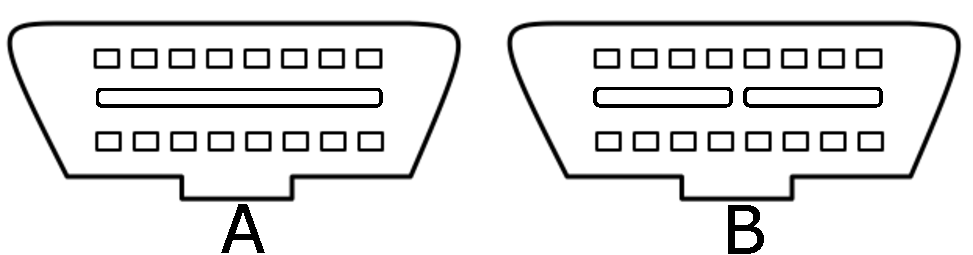
\includegraphics[scale=0.8]{Images/ZlaczaOBD2.pdf}
		\caption{Porównanie złącza diagnostycznego w wersji A oraz B.}
		\label{rys_obd2_wtyczka}
		\end{figure}
		
		Złącze typu A stosowane jest w pojazdach wyposażonych w akumulator o napięciu 12V, natomiast złącze typu B w pojazdach wyposażonych w akumulator o napięciu 24V.
		
		Norma SAE J1962 definiuje protokoły komunikacyjne udostępniane przez złącze diagnostyczne. Dostępność poszczególnych protokołów komunikacyjnych może być różna w zależności od producenta pojazdu oraz roku produkcji. Na Rys. \ref{rys_obd2_pinout} oraz w tabeli \ref{tab_obd2_pinout} przedstawione zostały potencjalnie dostępne protokoły komunikacyjne wraz z numerem pinu, do którego powinny być podłączone.
		
		\begin{figure}[ht]
		\centering
		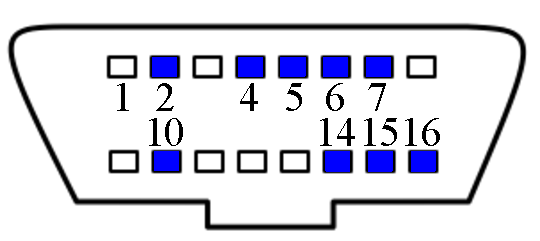
\includegraphics[scale=0.8]{Images/ZlaczeOBD2_pinout.pdf}
		\caption{Opis wyprowadzeń złącza diagnostycznego. Wykorzystywane wyprowadzenia zostały zaznaczone kolorem niebieskim oraz odpowiednim numerem. Opis wyprowadzeń znajduje się w Tab \ref{tab_obd2_pinout}}
		\label{rys_obd2_pinout}
		\end{figure}
		
		W złączu diagnostycznym udostępnionych jest 5 różnych protokołów. Dodatkowo rozróżnione są dwie masy: masa podwozia oraz masa sygnałowa. W praktyce najczęściej wyprowadzenia te są ze sobą zwarte. Zazwyczaj w pojazdach udostępniony jest tylko jeden z opisanych poniżej protokołów. 
		
		\newpage
		
		\begin{table}[ht]
\centering
\caption{Opis wyprowadzeń złącza diagnostycznego OBD-II.}
\label{tab_obd2_pinout}
\begin{tabular}{|c|c|}
\hline
\textbf{Numer wyprowadzenia} & \textbf{Przeznaczenie wyprowadzenia}                                                                    \\ \hline
2                            & Linia dodatnia protokołu SAE J1850 PWM oraz VPW                                                         \\ \hline
4                            & Masa podwozia                                                                                           \\ \hline
5                            & Masa sygnałowa                                                                                          \\ \hline
6                            & Linia wysoka magistrali CAN                                                                             \\ \hline
7                            & Linia K protokołu ISO 9141-2 oraz ISO 14230-4                                                           \\ \hline
10                           & Linia ujemna protokołu SAE J1850 PWM                                                                    \\ \hline
14                           & Linia niska magistrali CAN                                                                              \\ \hline
15                           & Linia L protokołu ISO 9141-2 oraz ISO 14230-4                                                           \\ \hline
16                           & \begin{tabular}[c]{@{}c@{}}Zasilanie\\ 12V/4A dla złącza typu A\\ 24V/2A dla złącza typu B\end{tabular} \\ \hline
\end{tabular}
\end{table}

		\subsubsection{Protokoły komunikacyjne dostępne w złączu diagnostycznym}
		\hspace{0.5cm}Zgodnie z normą SAE J1962 do złącza diagnostycznego doprowadzone może być pięć różnych magistral danych które udostępniają następujące protokołu komunikacji:
		
		\begin{itemize}
			\item{SAE J1850 PWM,}
			\item{SAE J1850 VPW,}
			\item{CAN,}
			\item{ISO 9141,}
			\item{ISO 14230 - KWP2000.}
		\end{itemize}
		
		\newpage
		
		\subsection{Struktura zapytań złącza diagnostycznego}
		
		\hspace{0.5cm}Zgodnie z normą SAE J1979 z komputerem pokładowym pojazdu można komunikować się poprzez złącze diagnostyczne wysyłając odpowiednie komendy. Mają one postać heksadecymalnego ciągu cyfr, a pojedyncze instrukcje komputera pokładowego kodowane są jako dwie cyfry. Kod zapytania musi składać się z przynajmniej dwóch znaków. Każda instrukcja powinna być zakończona znakiem powrotu karetki. Kody zapytań podzielone są na dziesięć grup zwanych modami pracy złącza diagnostycznego. Nagłówki zapytań dla poszczególnych modów wraz z ich opisem przedstawiono w tabeli \ref{tab_pid_modes}.
		
		\begin{table}[ht]
\centering
\caption{Tryby pracy złącza diagnostycznego}
\label{tab_pid_modes}
\begin{tabular}{|c|c|}
\hline
\textbf{Tryb (hex)} & \textbf{Opis}                                                               \\ \hline
01                  & Aktualny stan parametrów                              \\ \hline
02                  & Zapisane w pamięci stan parametrów                      \\ \hline
03                  & Wyświetlenie kodów błędów                                                        \\ \hline
04                  & Wyczyszczenie kodów błędów            \\ \hline
05                  & Wyniki testu czujników tlenu \\ \hline
06                  & Wyniki testu czujnika tlenu (CAN)                             \\ \hline
07                  & Wyświetlenie niepotwierdzonych kodów błędów         \\ \hline
08                  & Kontrola operacji poszczególnych układów wewnętrznych                       \\ \hline
09                  & Wyświetlanie informacji o pojeździe                                                           \\ \hline
0A                  & Trwałe kody błędów (czyste kody błędów)                                     \\ \hline
\end{tabular}
\end{table}

	

	W złączu diagnostycznym pojazdu nie muszą być udostępnione wszystkie mody pracy, a także nie muszą być udostępnione wszystkie kody zapytań z udostępnionego modu. Ogólna struktura kodów zapytań ma postać:

	\begin{itemize}
		\item{AA BB C,}
	\end{itemize}
		 gdzie AA to numer modu, BB to kod danego zapytania z wybranego modu natomiast C to liczba linii oczekiwanej odpowiedzi. Kody BB oraz C są opcjonalne, kod AA musi być zawarty w każdym zapytaniu. 
		 
		 Struktura odpowiedzi złącza diagnostycznego na zadany kod jest podobna do zapytania:
		
		\begin{itemize}
			\item{AA BB XX XX XX XX,}
		\end{itemize}		
		gdzie AA to wartość modu zapytania powiększona o 40, BB to powtórzenie kodu z zapytania, natomiast wartości XX XX XX XX to właściwa treść odpowiedzi. W zależności od wysłanego zapytania liczba bajtów odpowiedzi może być różna. Poniżej zaprezentowane zostało przykładowe zapytanie, wraz z przykładową odpowiedzią. 
		
		\begin{itemize}
			\item{01 00}
			\item{41 00 BE 1F B8 10}
		\end{itemize}
		
	\newpage		
		
		Interpretacja odpowiedzi jest różna w zależności od wysłanego zapytania. Powyższe zapytanie dotyczy kodów udostępnionych przez złącze diagnostyczne dla modu 01 z zakresu 01-20. Odpowiedź - po usunięciu z niej nagłówka - należy zapisać w postaci binarnej, w której wartość 1 oznacza że dany kod jest udostępniony. Interpretacja tego przykładu przedstawiona została w tabeli \ref{tab_pid_response}
		
\begin{table}[!h]
\centering
\caption{Interpretacja części odpowiedzi na kod zapytania 01 00}
\label{tab_pid_response}
\begin{tabular}{|c|c|c|c|c|c|c|c|c|c|c|}
\hline
\textbf{\begin{tabular}[c]{@{}c@{}}Bajt\\ odpowiedzi\\ (hex)\end{tabular}} & \multicolumn{4}{c|}{B} & \multicolumn{4}{c|}{E} & \textbf{.} & \textbf{.} \\ \hline
\textbf{\begin{tabular}[c]{@{}c@{}}Postać\\ binarna\end{tabular}}          & 1    & 0   & 1   & 1   & 1    & 1   & 1   & 0   & \textbf{.} & \textbf{.} \\ \hline
\textbf{Kod PID}                                                           & 01   & 02  & 03  & 04  & 05   & 06  & 07  & 08  & \textbf{.} & \textbf{.} \\ \hline
\end{tabular}
\end{table}		

		Pełna specyfikacja kodów zapytań oraz ich odpowiedzi zapisana jest w normie SAE J1979\cite{saej1979}.
		
		\newpage
		
		\subsection{Struktura kodów błędów}
		
		\hspace{0.5cm}Podstawową funkcjonalnością złącza diagnostycznego jest raportowanie błędów poszczególnych układów za pomocą diagnostycznych kodów błędów(ang. Diagnostic Trouble Codes - DTC). Aby uzyskać informację o zapisanych kodach należy wysłać zapytanie 03 do złącza diagnostycznego, ale najpierw zdefiniować ile kodów jest obecnych w pamięci. W tym celu należy wysłać komendę:
		
		\begin{itemize}
			\item{01 01.}
		\end{itemize}
		Kod odpowiedzi powinien mieć postać zbliżoną do: 

		\begin{itemize}
			\item{41 01 81 07 65 04.}
		\end{itemize}
		
		Wartości 41 01 to nagłówek odpowiedzi. Właściwa odpowiedź zaczyna się od dwóch pary bajtów 81, w których zapisana jest informacja o ilości przechowywanych kodów błędów pojazdu. Wartość 81 to liczba zapisana w postaci szesnastkowej, której wartość w systemie dziesiętnym to 129. Nie jest to jednak wprost liczba kodów błędów. W kodzie tym zawarta jest również informacja o stanie diody kontrolnej silnika, który zapisany jest na najbardziej znaczącym bicie, co oznacza, że odczytaną wartość należy pomniejszyć o 128 lub 80 w systemie szesnastkowym. Wynika z tego że w zaprezentowanym przykładzie przechowywany jest tylko jeden kod błędu. Podany przykład ilustruję sytuację, w której pojazd udostępnia tylko jeden moduł, który raportuje kody błędów. Jeżeli takich modułów byłoby więcej w odpowiedzi na instrukcję 01 01 wysłana zostanie odpowiedź podobna do przedstawionej dla każdego modułu. W celu sprawdzenia z którego modułu wysłana została odpowiedź należy włączyć wysyłanie nagłówka odpowiedzi.
		
		Po ustaleniu liczby przechowywanych błędów można przejść do odczytywania ich kodów poprzez wysłanie instrukcji 03. Odpowiedź powinna mieć postać zbliżoną do:
		
		\begin{itemize}
			\item{43 01 33 00 00 00 00.}
		\end{itemize}
		
		Wartość 43 to nagłówek odpowiedzi na kod 03. Kolejnych 6 bajtów powinno być odczytywanych parami. Każda para reprezentuje jeden kod błędu. W powyższym przypadku przechowywany jest tylko jeden kod 0133, natomiast zgodnie z standardem SAE odpowiedź została uzupełniona bajtami 00, które nie są interpretowane jako kody diagnostyczne. Pierwsza cyfra w odczytanym kodzie zawsze przechowuje zakodowaną informację o źródle błędu. Sposób dekodowania źródła wystąpienia błędu przedstawiony został w tabeli \ref{tab_dtc_interpret}.
		
		\newpage
		
		
		
	
		\newpage	
	
	\subsection{Opis wykorzystanych narzędzi}
		\hspace{0.5cm}
		-java
		-javafx
		-raspberry
		-PCB
		-maven
		-ELM327
	
		\newpage
	
%---------------------------------------------------STRUKTURA PROJEKTU-------------------------------------------------------------	
\section{Struktura projektu}
	\hspace{0.5cm}
	-założenia całościowe
	-schemat
	-opis ogólny	
	
	\newpage	
	
%---------------------------------------------------PROJEKT PŁYTKI-------------------------------------------------------------	
\section{Projekt układu do komunikacji ze złączem diagnostycznym}
	\subsection{Zastosowane elementy}W projekcie układu do komunikacji ze złączem diagnostycznym wykorzystane zostały układy scalone wymienione poniżej(w nawiasie znajduje się symbol odpowiadający danemu elementowi na Rys. \ref{rys_schemat_ukladu_elektrycznego}.
	
	\begin{itemize}
		\item{Mikroprocesor F103CBT6 firmy STM32(U1). W tabeli \ref{tab_stm32} przedstawione zostały jego najważniejsze w kontekście omawianego układu dane katalogowe.
			\begin{table}[!h]
			\centering
			\caption{Najważniejsze parametry STM32F103CBT6 \cite{stm32}.}
			\label{tab_stm32}
			\begin{tabular}{|c|c|c|c|}
			\hline
			\textbf{\begin{tabular}[c]{@{}c@{}}Napięcie\\ zasilania\end{tabular}} & \textbf{\begin{tabular}[c]{@{}c@{}}Częstotliwość\\ Taktowania\end{tabular}} & \textbf{\begin{tabular}[c]{@{}c@{}}Pamięć\\ Flash\end{tabular}} & \textbf{\begin{tabular}[c]{@{}c@{}}Pamięć\\ SRAM\end{tabular}} \\ \hline
3.3V & 72MHz & 128kB  & 20kB \\ \hline \hline 
\textbf{\begin{tabular}[c]{@{}c@{}}Liczba\\ timerów\end{tabular}} & \textbf{Interfejsy} & \textbf{Obudowa} & \textbf{Montaż}\\ \hline 
4, 16bit & \begin{tabular}[c]{@{}c@{}}CAN, I2C x2, LIN\\ SPI x2, USART x2\end{tabular} & LQFP48 & SMD \\ \hline
	\end{tabular}
	\end{table}
		}
		
		\item{Moduł komunikacji bluetooth RN4020-V/RM firmy Microchip(U2). W tabeli \ref{tab_RN4020} przedstawione zostały jego najważniejsze dane katalogowe.
		
		\begin{table}[!h]
		\centering
		\caption{Najważniejsze parametry RN4020-V/RM \cite{RN4020}.}
		\label{tab_RN4020}
		\begin{tabular}{|c|c|c|c|}
		\hline
\textbf{\begin{tabular}[c]{@{}c@{}}Napięcie\\ zasilania\end{tabular}} & \textbf{Standard}                                                      & \textbf{Komunikacja}                                                & \textbf{Protokół}                                           \\ \hline
3.0-3.6V                                                              & 4.1                                                                    & UART                                                                & \begin{tabular}[c]{@{}c@{}}ASCII AT\\ Commands\end{tabular} \\ \hline \hline
\textbf{\begin{tabular}[c]{@{}c@{}}Programowalne\\ GPIO\end{tabular}} & \textbf{\begin{tabular}[c]{@{}c@{}}Częstotliwość\\ pracy\end{tabular}} & \textbf{\begin{tabular}[c]{@{}c@{}}Wbudowana\\ antena\end{tabular}} & \textbf{Montaż}                                             \\ \hline
\begin{tabular}[c]{@{}c@{}}7 cyfrowych\\ 3 analogowe\end{tabular}                                                                  & 2.402-2.480GHz                                                         & Tak                                                                 & SMD                                                         \\ \hline
\end{tabular}
\end{table}
		
		}		
	
	\item{Interfejs protokołu ISO9141-2, L9637D firmy STMicroelectronics(U3). Dane katalogowe tego układu znaleźć można w odnośniku \cite{L9637D}.}
	\item{Regulator napięcia 5V MC7805BDTRK(U4). Dane katalogowe tego układu znaleźć można w odnośniku \cite{MC7805}.}
	
	\item{Regulator napięcia 3V MCP1703T-3302E/CB(U5). Dane katalogowe tego układu znaleźć można w odnośniku \cite{MCP17}.}
	
	\end{itemize}	
	
	\newpage
	
	W tabeli \ref{tab_wykaz_czesci} znajduje się pełny wykaz wykorzystanych elementów.
	
	\begin{table}[!h]
\centering
\caption{Wykaz wykorzystanych elementów wraz z opisem obudowy, rodzaju montażu oraz warstwy na projekcie obwodu drukowanego.}
\label{tab_wykaz_czesci}
\begin{tabular}{|c|c|c|c|c|c|}
\hline
\textbf{Oznaczenie} & \textbf{Nazwa/wartość} & \textbf{Obudowa} & \textbf{Montaż} & \textbf{Ilość} & \textbf{Warstwa} \\ \hline
U1                  & STM32F103CBT6          & LQFP48           & SMD             & 1              & Górna            \\ \hline
U2                  & RN4020-V/RM            & RN4020-ALT       & SMD             & 1              & Dolna            \\ \hline
U3                  & L9637D                 & SO8              & SMD             & 1              & Górna            \\ \hline
U4                  & \begin{tabular}[c]{@{}c@{}}MC78M05\\ BDTRK\end{tabular}           & TO-252-3  & SMD             & 1              & Górna            \\ \hline
U5                  & \begin{tabular}[c]{@{}c@{}}MCP1703T-3302\\ E/CB\end{tabular}      & SOT-23-3         & SMD             & 1              & Górna            \\ \hline
R1, R2, R3          & 330$\Omega$                   & 0402             & SMD             & 3              & Dolna            \\ \hline
R4, R5              & 330$\Omega$                   & 0402             & SMD             & 2              & Górna            \\ \hline
R7                  & 510$\Omega$                   & 0402             & SMD             & 1              & Górna            \\ \hline
R8                  & 12k$\Omega$                   & 0402             & SMD             & 1              & Górna            \\ \hline
R9                  & 22k$\Omega$                   & 0402             & SMD             & 1              & Górna            \\ \hline
R10                 & 1M$\Omega$                    & 0402             & SMD             & 1              & Dolna            \\ \hline
R11                 & 10k$\Omega$                   & 0402             & SMD             & 1              & Dolna            \\ \hline
C1, C2, C12         & 1$\mu$F 16V                & 0402             & SMD             & 3              & Górna            \\ \hline
C3                  & 1$\mu$F 25V                & 0603             & SMD             & 1              & Górna            \\ \hline
C5                  & 100nF 16V              & 0402             & SMD             & 1              & Dolna            \\ \hline
C6                  & 100nF 16V              & 0402             & SMD             & 1              & Górna            \\ \hline
C7, C8              & 22pF 50V               & 0402             & SMD             & 2              & Dolna            \\ \hline
C9, C10             & 10pF 50V               & 0402             & SMD             & 2              & Dolna            \\ \hline
C11                 & 4.7$\mu$F 10V              & 0402             & SMD             & 1              & Dolna            \\ \hline
D1, D2, D3          & Red diode              & 0402             & SMD             & 3              & Dolna            \\ \hline
D4, D5              & Red diode              & 0402             & SMD             & 2              & Górna            \\ \hline
D8                  & 1N4007                 & DO-41            & THT             & 1              & Górna            \\ \hline
Q1                  & 32.768kHz              & 3.2x1.5x0.9    & SMD             & 1              & Dolna            \\ \hline
Q2                  & 8MHz                   & HC49U            & THT             & 1              & Dolna            \\ \hline
P1                  & Header                 & HDR1X4           & THT             & 1              & Górna            \\ \hline
P3                  & Header                 & HDR1X5           & SMD             & 1              & Górna            \\ \hline
P4                  & Header                 & HDR1X3           & THT             & 1              & Górna            \\ \hline
S1                  & Button PS-03B          & SPST-NO          & THT             & 1              & Górna            \\ \hline
CB1                 & Button PS11ABK         & SPST-NO          & THT             & 1              & Górna            \\ \hline
\end{tabular}
\end{table}

\newpage
	
	\newpage
	\subsection{Schemat elektryczny}
	
		\hspace{0.5cm}Celem zaprojektowanego układu było umożliwienie komunikacji z samochodowym komputerem pokładowym poprzez złącze diagnostyczne. Głównym elementem układu jest mikroprocesor U1, którego zadaniem jest odbieranie danych ze złącza diagnostycznego oraz przesyłanie odebranych danych za pomocą modułu bluetooth do układu wizualizacji danych. Mikroprocesor zasilany jest napięciem 3.3V. Układ został zaprojektowany do obsługi tylko jednego protokołu komunikacyjnego udostępnianego przez złącze diagnostyczne - ISO 9141-2. Wynika to z potrzeby minimalizacji całego układu, a także minimalizacji ceny jego wykonania. Sygnał protokołu komunikacyjnego doprowadzony jest do złącza P1 wraz z napięciem 12V - którego źródłem jest akumulator - oraz wyprowadzeniami masy układu. Sygnał zasilania złącza P1 doprowadzony jest to dwóch regulatorów napięcia U4 oraz U5, dzięki którym w układzie dostępne są napięcia zasilające odpowiednio 5V oraz 3.3V. W obwodzie wejściowym oraz wyjściowym umieszczone zostały kondensatory C1, C2 i C3 zgodnie z zaleceniami producenta \cite{MC7805}\cite{MCP17}. W obwodzie zasilania znajduje się dioda prostownicza D8 oraz dodatkowo dwie czerwone diody LED D4 i D5 wraz z odpowiadającymi im rezystorami R4 i R5, których zadaniem jest sygnalizowanie obecności napięcia.
		
		Sygnał linii k protokołu ISO 9141-2 wychodzący ze złącza P1 doprowadzony jest do układu interfejsu magistrali ISO 9141. Układ ten zasilany jest napięciem 5V, a jego zadaniem jest przetwarzanie sygnału wyprowadzonego ze złącza diagnostycznego. Zastosowanie takiego rozwiązania umożliwia wygodne programowanie komunikacji ze złączem diagnostycznym przy użyciu interfejsu UART, które  jest bezpośrednio dostępne w zastosowanym mikroprocesorze. Ze względu na różnicę napięć pracy układu L9637D oraz mikroprocesora do odbierania danych z wyprowadzenia Rx interfejsu ISO należy dodatkowo obniżyć napięcie sygnału. Do tego celu wykorzystano rezystancyjny dzielnik napięcia R8 i R9. Wysyłanie danych z mikroprocesora może odbywać się bezpośrednio, ponieważ napięcie 3.3V jest wystarczające do zmiany stanu na wejściu Tx układu U3. W obwodzie komunikacji pomiędzy modułami umieszczono dodatkowo złącze umożliwiające bezpośrednie odczytywanie danych na liniach Rx oraz Tx, które może być wykorzystywane w celach diagnostycznych lub jako wyprowadzenie do dodatkowego mikroprocesora. Dokładny opis układu można znaleźć w nocie katalogowej producenta \cite{L9637D}.
		
		Układ U2 znajdujący się na schemacie to moduł komunikacyjny bluetooth. Jego zadaniem jest odbieranie wstępnie opracowanych wyników ze złącza diagnostycznego do układu wizualizacji danych. Moduł charakteryzuje się małym poborem prądu w stanie pracy(12mA), bardzo małym w stanie spoczynku(<0.5A), a także dużą szybkością przesyłania danych(do 1Mbps). Dokładną specyfikację urządzenia można znaleźć w nocie katalogowej producenta \cite{RN4020}. Układ zasilany jest napięciem 3.3V oraz komunikuje się z mikroprocesorem wykorzystując magistralę UART. Dodatkowo do modułu U2 doprowadzony jest sygnał wybudzający ze stanu czuwania(7:WAKE\_ SW) oraz sygnał wejścia resetującego układ(8:CMD/MLDP). Wyprowadzenia PIO1, PIO2, PIO3 wykorzystane zostały do sygnalizowania stanu komunikacji układu. Dodatkowo moduł bluetooth posiada wyprowadzenia magistrali SPI, które w zaprojektowanym układzie nie zostały wykorzystane. 
		
		\newpage		
		
		W układzie znajdują się również elementu obsługi mikroprocesora. Złącze P3 umożliwia programowanie mikroprocesora z wykorzystaniem zewnętrznego programatora dostępnego w zestawach STM32 NUCLEO lub DISCOVERY lub programatora ST-LINK/V2. Dodatkowo w układzie znajdują się dwa rezonatory kwarcowe(Q1, Q2) wraz kondensatorami(C7, C8, C9, C10) zgodne z zaleceniami producenta, a także przycisk umożliwiający resetowanie układu(S1). 
		
		Rys. \ref{rys_schemat_ukladu_elektrycznego} przedstawia schemat zaprojektowanego układu. Schemat w większym rozmiarze dodany został również do załączników na końcu dokumentu.
		
		\begin{figure}[!h]
			\centering
			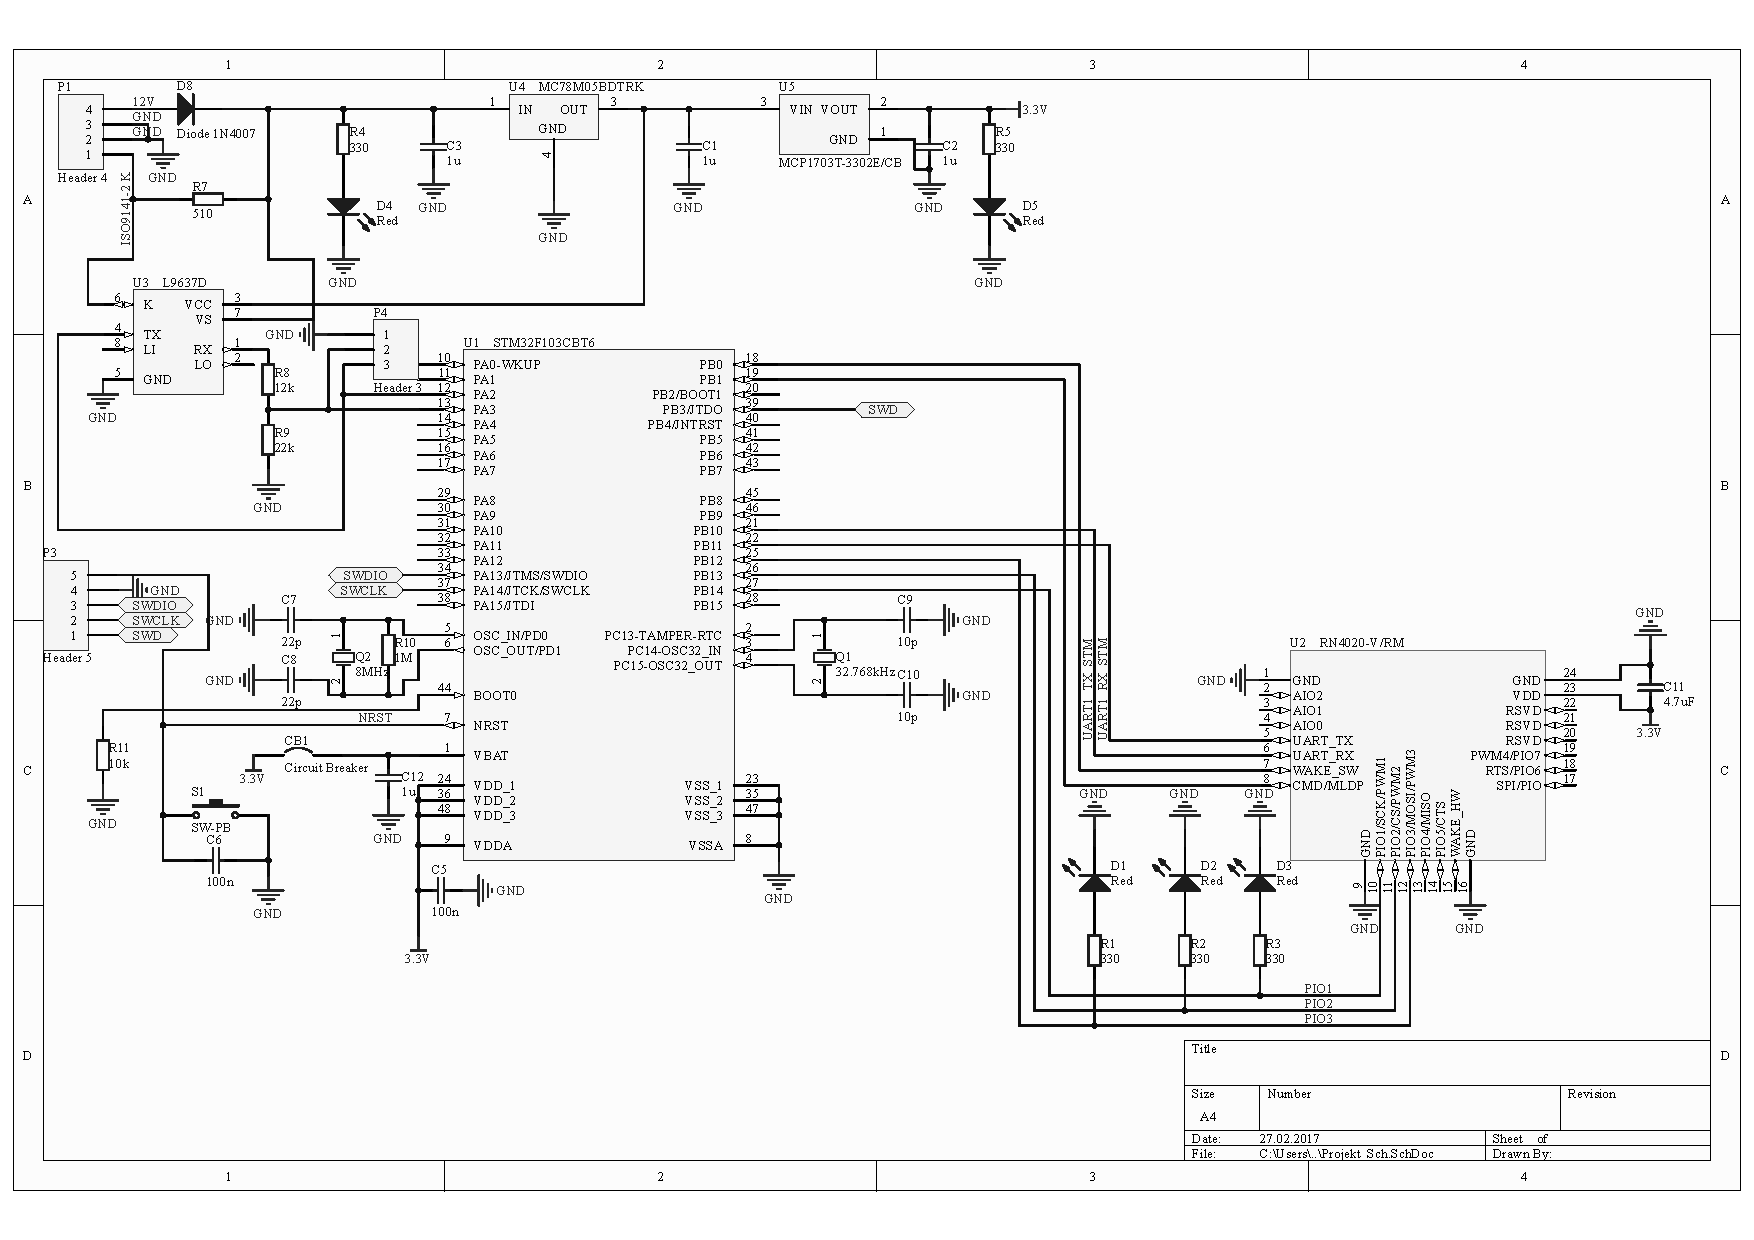
\includegraphics[scale=0.6, angle=90]{Images/SchematUkladuElektrycznego.pdf}
			\caption{Schemat obwodu układu do komunikacji ze złączem diagnostycznym. Opis w tekście.}
			\label{rys_schemat_ukladu_elektrycznego}
		\end{figure}
	
		\newpage
	
	\subsection{Projekt obwodu drukowanego}
		\hspace{0.5cm}Na podstawie zaprojektowanego schematu elektrycznego zaprojektowany został obwód drukowany. Przy projektowaniu istotnym aspektem był rozmiar oraz kształt wykonanej płytki, aby układ mógł zostać umieszczony w obudowie, której widok oraz przekrój poprzeczny wraz z wymiarami przedstawiony został na Rys. \ref{widok_wtyczka_obd}.
		
		\begin{figure}[!h]
			\centering
			\subfigure[]{
				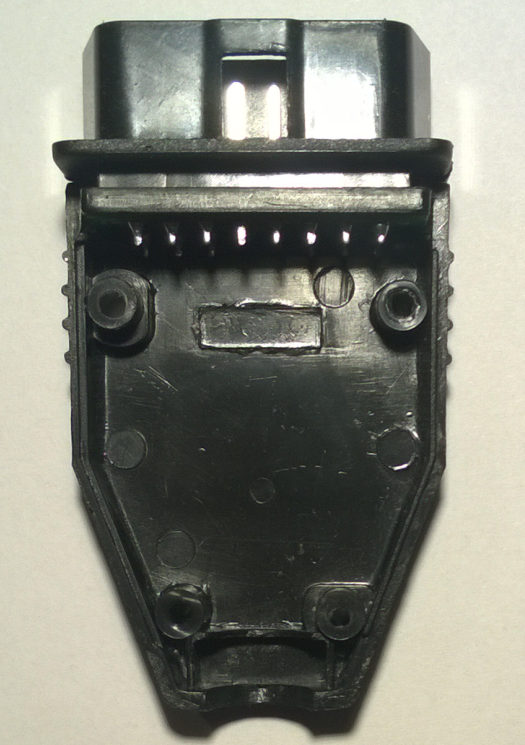
\includegraphics[scale=0.3]{Images/widok_wtyczka_obd.png}
			} 
			\subfigure[]{
				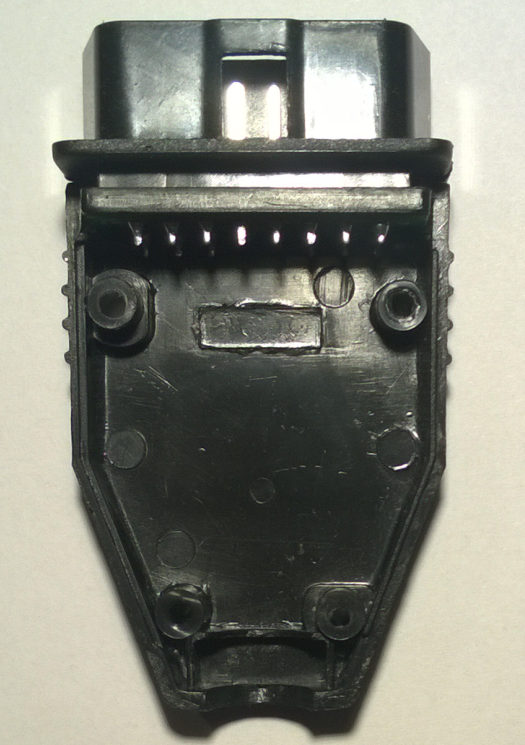
\includegraphics[scale=0.3]{Images/widok_wtyczka_obd.png}
			} 
			\caption{Widok (a) oraz przekrój poprzeczny z wymiarami (b) obudowy układu do komunikacji ze złączem diagnostycznym.}
			\label{widok_wtyczka_obd}
		\end{figure} 
	
	Projekt obwodu drukowanego został wykonany w technologii dwustronnej. W tabeli \ref{tab_opis_warstw_pcb} znajduje się opis poszczególnych warstw zaprojektowanej płytki.
	
	\begin{table}[!h]
\centering
\caption{Opis wykorzystanych warstw.}
\label{tab_opis_warstw_pcb}
\begin{tabular}{|c|c|c|c|}
\hline
\textbf{Nazwa/Typ}                                                & \textbf{Materiał}                                         & \textbf{Grubość {[}mm{]}} & \textbf{\begin{tabular}[c]{@{}c@{}}Stała\\ dielektryczna\end{tabular}} \\ \hline
Pokrycie górne                                                    &                                                           &                           &                                                                        \\ \hline
Górna soldermaska                                                 & Poliamid                                                  & 0.01016                   & 3.5                                                                    \\ \hline
\begin{tabular}[c]{@{}c@{}}Górna warstwa\\ sygnałowa\end{tabular} & Miedź                                                     & 0.03556                   &                                                                        \\ \hline
\begin{tabular}[c]{@{}c@{}}Warstwa\\ dielektryczna\end{tabular}   & \begin{tabular}[c]{@{}c@{}}Dielektryk\\ FR-4\end{tabular} & 0.32004                   & 4.8                                                                    \\ \hline
\begin{tabular}[c]{@{}c@{}}Dolna warstwa\\ Sygnałowa\end{tabular} & Miedź                                                     & 0.03556                   &                                                                        \\ \hline
Dolna soldermaska                                                 & Poliamid                                                  & 0.01016                   & 3.5                                                                    \\ \hline
Pokrycie dolne                                                    &                                                           &                           &                                                                        \\ \hline
\end{tabular}
\end{table}

		\newpage
	
		W tabeli \ref{tab_wykaz_czesci}	znajduje się wykaz zastosowanych elementów wraz z warstwą, na której zostały umieszczone. Na Rys. \ref{warstwa_top} \ref{warstwa_bottom} przedstawione zostały schematy obwodów obu warstw, a także widoki modelu. 
	
		\begin{figure}[!h]
			\centering
			\subfigure[]{
				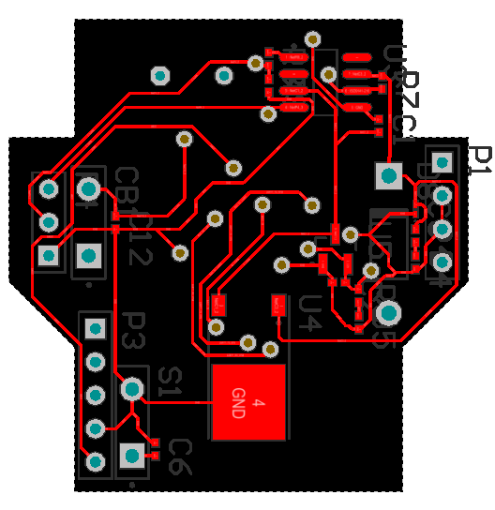
\includegraphics[scale=0.4]{Images/rys_pcb_top_schemat.png}
			} 
			\subfigure[]{
				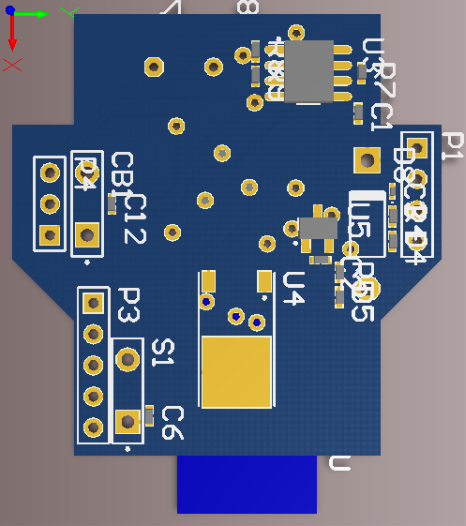
\includegraphics[scale=0.4]{Images/rys_pcb_top_model.png}
			} 
			\caption{Schemat obwodu (a) oraz widok modelu (b) górnej warstwy płytki.}
			\label{warstwa_top}
		\end{figure} 		
		
		\begin{figure}[!h]
			\centering
			\subfigure[]{
				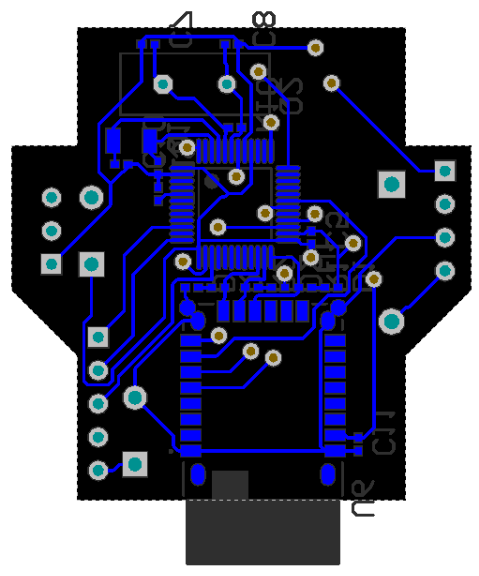
\includegraphics[scale=0.4]{Images/rys_pcb_bottom_schemat.png}
			} 
			\subfigure[]{
				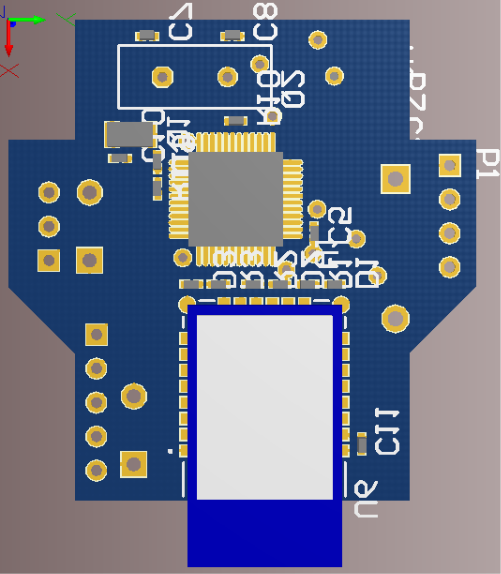
\includegraphics[scale=0.4]{Images/rys_pcb_bottom_model.png}
			} 
			\caption{Schemat obwodu (a) oraz widok modelu (b) dolnej warstwy płytki.}
			\label{warstwa_bottom}
		\end{figure} 
		
		\newpage
		
		
	
		\newpage
%---------------------------------------------------APLIKACJA KOMUNIKACYJNA-------------------------------------------------------------	
	
\section{Aplikacja przetwarzająca dane ze złącza diagnostycznego}
	\hspace{0.5cm}
	
	\newpage
	
%---------------------------------------------------INTERFEJS GRAFICZNY-------------------------------------------------------------	
	
\section{Interfejs użytkownika}
	\hspace{0.5cm}
	
	\newpage
	
\section{Podsumowanie}
	
	\hspace{0.5cm} 
	
	\newpage	
	
\begin{thebibliography}{99}

		\bibitem{Massalski80}
		Massalski J., Massalska M., \emph{Fizyka dla inżynierów część I}, Wydawnictwo Naukowo-Techniczne, Warszawa, 1980.
	
		\bibitem{Halliday12}
		Halliday D., Resnick R., Walker J., \emph{Podstawy fizyki tom 2}, Wydawnictwo Naukowe PWN, Warszawa, 2012.

		\bibitem{Sawieliew98}
		Sawieliew I. W., \emph{Wykład z fizyki tom 1}, Wydawnictwo Naukowe PWN, Warszawa, 2002.
	
		\bibitem{Bogusz10}
		Bogusz W., Grabarczyk J., Krok F., \emph{Podstawy fizyki}, Oficyna Wydawnicza Politechniki Warszawskiej, Warszawa, 2010.
		
		\bibitem{saej1962}
		https://law.resource.org/pub/us/cfr/ibr/005/sae.j1962.2002.pdf (14.02.2017)
		
		\bibitem{saej1979}
		https://law.resource.org/pub/us/cfr/ibr/005/sae.j1979.2002.pdf (14.02.2017)
		
		\bibitem{stm32}
		http://www.st.com/content/ccc/resource/technical/document/datasheet/33/d4/6f/
		1d/df/0b/4c/6d/CD00161566.pdf/files/CD00161566.pdf/jcr:content/translations/
		en.CD00161566.pdf (27.02.2017)
		
		\bibitem{RN4020}
		http://ww1.microchip.com/downloads/en/DeviceDoc/50002279A.pdf (27.02.2017)
		
		\bibitem{L9637D}
		http://www.st.com/content/ccc/resource/technical/document/datasheet/4a/80/83/
		26/e0/78/4d/18/CD00000234.pdf/files/CD00000234.pdf/jcr:content/translations/
		en.CD00000234.pdf (27.02.2017)
		
		\bibitem{MC7805}
		http://pdf.datasheetcatalog.com/datasheet2/9/0p4t1g1lw0spoo5ukh2s1uxchzky.pdf (27.02.2017)
		
		\bibitem{MCP17}
		http://www.mouser.com/ds/2/268/22049a-51817.pdf (27.02.2017)
		

\end{thebibliography}
	\newpage

	\listoffigures{}
	\newpage

	\listoftables
	\newpage

\end{document}